%%%%%%%%%%%%%%%%%%%%%%%%%%%%%%%%%%%%%%%%%%%%%%%%%%%%%%%%%%%%%%%%%%%%%%%%

%%% AAMAS 2027 working manuscript derived from the official sample.
%%% The class, copyright block, and layout parameters are unchanged.
%%% Editorial reference: best-paper-writing-guide.md. Pending numerical
%%% results are documented in comments; author instructions stay out of the PDF.

%%%%%%%%%%%%%%%%%%%%%%%%%%%%%%%%%%%%%%%%%%%%%%%%%%%%%%%%%%%%%%%%%%%%%%%%

%%% Use the first variant for double-blind review and the second only for
%%% the camera-ready paper.

\documentclass[sigconf,anonymous]{aamas}
%\documentclass[sigconf]{aamas}

% Start final-column balancing explicitly on the last page.  The class hook
% otherwise runs after the bibliography and can strand the end of a DOI.
\makeatletter
\@ACM@balancefalse
\makeatother

\usepackage{balance}
\usepackage{xspace}
\usepackage{algorithm}
\usepackage{algpseudocode}
\usepackage{tikz}
\usetikzlibrary{arrows.meta,positioning}
\algrenewcommand\algorithmicrequire{\textbf{Input:}}
\algrenewcommand\algorithmicensure{\textbf{Output:}}

%%%%%%%%%%%%%%%%%%%%%%%%%%%%%%%%%%%%%%%%%%%%%%%%%%%%%%%%%%%%%%%%%%%%%%%%

%%% AAMAS-2027 copyright block (do not change!)

\makeatletter
\gdef\@copyrightpermission{
  \begin{minipage}{0.2\columnwidth}
   \href{https://creativecommons.org/licenses/by/4.0/}{
\includegraphics[width=0.90\textwidth]{by}}
  \end{minipage}\hfill
  \begin{minipage}{0.8\columnwidth}
   \href{https://creativecommons.org/licenses/by/4.0/}{This work is licensed under a Creative Commons Attribution International 4.0 License.}
  \end{minipage}
  \vspace{5pt}
}
\makeatother

\setcopyright{ifaamas}
\acmConference[AAMAS 2027]{Proc.\@ of the 26th International Conference
on Autonomous Agents and Multiagent Systems (AAMAS 2027)}{3--7 May 2027}{Hanoi, Vietnam}{M.~Baldoni, F.~Fang, W.~Yeoh, N.~Yorke-Smith (eds.)}
\copyrightyear{2027}
\acmYear{2027}
\acmDOI{}
%\acmPrice{}
\acmISBN{}

%%%%%%%%%%%%%%%%%%%%%%%%%%%%%%%%%%%%%%%%%%%%%%%%%%%%%%%%%%%%%%%%%%%%%%%%

\acmSubmissionID{}
\submissionType{Research Paper Track}

\title[Decompose, Refine, and Reconstruct for HCP]{Decompose, Refine, and Reconstruct:\texorpdfstring{\\}{ }Structure-Aware SAT--CEGAR for the Hamiltonian Cycle Problem}

%%% The anonymous document class suppresses the following identifying data in
%%% the review PDF. Do not include this source file in an anonymous supplement.
\author{Quan Van Vi}
\affiliation{
  \institution{Vietnam National University, Hanoi}
  \city{Hanoi}
  \country{Vietnam}}
\email{22021149@vnu.edu.vn}

\author{Tuyen Van Kieu}
\affiliation{
  \institution{Vietnam National University, Hanoi}
  \city{Hanoi}
  \country{Vietnam}}
\email{tuyenkv@vnu.edu.vn}

\author{Khanh Van To}
\affiliation{
  \institution{Vietnam National University, Hanoi}
  \city{Hanoi}
  \country{Vietnam}}
\email{khanhtv@vnu.edu.vn}

%%%%%%%%%%%%%%%%%%%%%%%%%%%%%%%%%%%%%%%%%%%%%%%%%%%%%%%%%%%%%%%%%%%%%%%%

\newcommand{\BibTeX}{\rm B\kern-.05em{\sc i\kern-.025em b}\kern-.08em\TeX}
\newcommand{\sat}{\textsc{sat}}
\newcommand{\hcp}{\textsc{hcp}}
\newcommand{\cegar}{\textsc{cegar}}
\newcommand{\method}{\textsc{StructHCP}\xspace}

%%%%%%%%%%%%%%%%%%%%%%%%%%%%%%%%%%%%%%%%%%%%%%%%%%%%%%%%%%%%%%%%%%%%%%%%

\begin{abstract}
We present \method, a SAT-based solver for Hamiltonian cycle instances
whose construction leaves exploitable graph structure. The solver first
applies sound infeasibility filters and dispatches recognizable
hub--cluster, alternating-pair, and cubic graphs to tailored encodings.
For the remaining inputs, it performs SPQR-inspired reductions: maximal
degree-two chains are represented by forced virtual edges, components
behind a two-vertex separator are solved as endpoint-constrained paths,
and those paths are substituted into a smaller skeleton. A single
incremental SAT--CEGAR engine supports both cycle and path search by
refining disconnected cycle covers with cut-set clauses. All virtual
edges carry reconstruction maps, and a candidate is accepted only after
expansion and verification against the original graph. The unified Rust
implementation derives every decision from the input adjacency relation;
it contains no cached paths, injected tours, or graph-identifier routing.
On a 29-instance residual subset of the 1,001-instance FHCP Challenge
Set, we report 11 independently verified Hamiltonian-cycle certificates,
reducing the unresolved subset by 37.9\%. Each instance times out in all
21 archived SAT-based and reference configurations. The set includes
\texttt{graph788}, uniquely identified by its order and size as Sted6,
which no submission to the original FHCP Challenge solved. This is a
certificate-coverage result; the matched full-suite runtime comparison
is still in progress.
\end{abstract}

\begin{CCSXML}
<ccs2012>
 <concept>
  <concept_id>10010147.10010178.10010187</concept_id>
  <concept_desc>Computing methodologies~Discrete space search</concept_desc>
  <concept_significance>500</concept_significance>
 </concept>
</ccs2012>
\end{CCSXML}
\ccsdesc[500]{Computing methodologies~Discrete space search}
\keywords{Hamiltonian cycle problem, SAT, CEGAR, graph decomposition}

\begin{document}
\maketitle

\section{Introduction}
\label{sec:introduction}

The Hamiltonian cycle problem (HCP) asks whether an undirected graph
contains a simple cycle that visits every vertex exactly once. It is a
classical NP-complete problem~\cite{karp1972} and a useful test case for
combining local propagation with global connectivity. A compact
edge-variable SAT encoding enforces exactly two selected incident edges
at every vertex. Its models are cycle covers, however, so the encoding
must also eliminate disconnected subtours.

Counterexample-guided abstraction refinement (CEGAR) addresses this gap
by alternating between a relaxed SAT formula and connectivity constraints
learned from its models
~\cite{clarke2000cegar,soh2014incremental,ohashi2025cutset}. On large
structured graphs, a monolithic encoding repeatedly rediscovers local
choices whose interaction with the rest of the graph is confined to a
small interface. Degree-two chains are the simplest example: all of their
edges are forced, yet their internal vertices increase the encoding and
create additional subtours. Separation pairs and repeated hub--cluster
structure expose the same opportunity at a coarser scale. Cubic graphs
offer a different simplification: a directed one-in/one-out encoding
with explicit two-loop prohibition avoids symmetric undirected choices.

We present \method, organized around three operations: decompose the
input into sound path and skeleton subproblems, refine SAT cycle covers
incrementally, and reconstruct a cycle in the original graph. The new
implementation uses one CEGAR engine for ordinary cycles,
endpoint-constrained paths, and reduced skeletons. Its structural core
implements the series and separation-pair cases motivated by SPQR
decomposition, without claiming to construct a complete canonical SPQR
tree. Tailored hub--cluster, alternating-pair, and cubic front ends
remain certificate-producing accelerators. Except for the exact cubic
encoding, failure in a tailored front end simply transfers control to
the general reduction and CEGAR pipeline.

The implementation consumes a raw graph and constructs every local path
de novo. It does not read cached paths, stored cycle covers, reference
tours, or graph-specific vertex arrays. Routing depends on
adjacency-derived predicates rather than instance identifiers. Every
candidate is expanded and checked on the original graph before it can be
reported.

Our empirical focus is a 29-instance residual set from the 1,001
known-Hamiltonian graphs of the FHCP Challenge Set
~\cite{haythorpe2018fhcp}. The principal result is
\textbf{11 additional verified certificates}: every corresponding
instance is a timeout in all 21 configurations contained in the archived
baseline results. This resolves 37.9\% of the residual set. The set
includes \texttt{graph788}, whose unique vertex and edge counts identify
it as Sted6, one of 16 instances that no original challenge submission
solved~\cite{haythorpe2018fhcp,haythorpe2019change}. We separate this
certificate-coverage result from the full matched runtime study, which is
still running.

The contributions are:
\begin{itemize}
  \item sound series contraction and separation-pair path substitution
  with explicit reconstruction maps;
  \item a unified incremental SAT--CEGAR engine for cycles and endpoint
  paths, plus protected repair and a directed cubic encoding;
  \item a pure-Rust solver with adjacency-based dispatch, preemptive
  termination, and original-graph verification; and
  \item 11 verified solutions on the residual-29 set, including Sted6
  (\texttt{graph788}), extending both the archived baseline coverage and,
  for at least this instance, the original challenge coverage.
\end{itemize}

\section{Preliminaries}
\label{sec:preliminaries}

Let $G=(V,E)$ be a finite undirected simple graph, with $n=|V|\geq3$.
For $S\subseteq V$, let $\delta_G(S)$ contain the edges with exactly
one endpoint in $S$, and write $\delta_G(v)$ for the edges incident to
$v$. Associate a Boolean variable $x_e$ with each edge. The degree
formula
\begin{equation}
  \Phi_{\mathrm{deg}}(G)=
  \bigwedge_{v\in V}
  \left(\sum_{e\in\delta_G(v)}x_e=2\right)
  \label{eq:degree}
\end{equation}
describes a collection of vertex-disjoint cycles covering $V$. A model
is Hamiltonian exactly when this collection has one component.

For every nonempty proper $S\subset V$, a Hamiltonian cycle satisfies
\begin{equation}
  \sum_{e\in\delta_G(S)}x_e\geq2.
  \label{eq:cutset}
\end{equation}
Under Equation~\eqref{eq:degree}, every selected cut has even
cardinality. Consequently, the clause
$\bigvee_{e\in\delta_G(S)}x_e$ rules out a closed subtour on $S$ and
implies Equation~\eqref{eq:cutset} at the model level. We also use the
exact-cycle blocking clause
$\bigvee_{e\in E(C)}\neg x_e$. CEGAR starts from the degree formula,
decodes a model into cycles, and adds these clauses for proper cycles
until it finds one spanning cycle or proves the refined formula
unsatisfiable.

A spanning $s$--$t$ path through a vertex set $M$ uses degree one at
$s,t$ and degree two at every other vertex of $M$. The corresponding
relaxation may contain the endpoint path plus disjoint cycles; the
same refinement principle removes those cycles. This local primitive
is used by the structural solvers below.

\section{Method}
\label{sec:method}

\subsection{Overview}
\label{sec:overview}

Figure~\ref{fig:pipeline} shows the implemented control flow. Four
necessary-condition checks first reject graphs that are disconnected,
have minimum degree below two, contain an articulation vertex, or are
bipartite with unequal color classes. The solver then tests three
recognizers in order: hub--cluster, alternating pairs, and 3-regular
cubic structure. A recognized hub or alternating instance is offered to
a certificate-producing macro solver; failure continues to the general
pipeline. The cubic encoding is a complete decision procedure within
its time budget, so it may also report UNSAT.

The general pipeline contracts degree-two series chains, repeatedly
substitutes solved components behind separation pairs, solves the
remaining skeleton with the unified CEGAR engine, reverses every
substitution, and verifies the reconstructed tour. We call these
\emph{SPQR-inspired} reductions because they realize series (S) and
parallel/separation-pair (P) cases of triconnected decomposition
~\cite{hopcroft1973triconnected,dibattista1996spqr}. The implementation does not construct
or canonicalize a full SPQR tree and does not claim its linear-time
complexity.

\begin{figure}[t]
  \centering
  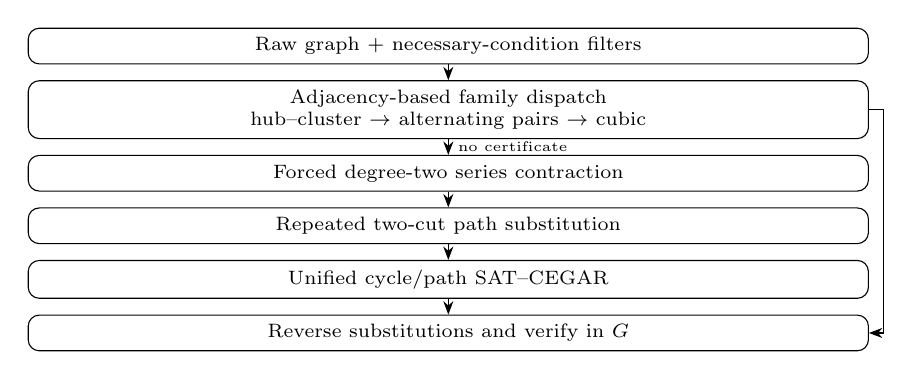
\begin{tikzpicture}[
    node distance=2.0mm,
    box/.style={draw,rounded corners,align=center,font=\scriptsize,
      minimum width=.88\columnwidth,minimum height=4.5mm},
    arrow/.style={-{Stealth[length=1.7mm]},thin}]
    \node[box] (input) {Raw graph + necessary-condition filters};
    \node[box,below=of input] (dispatch) {Adjacency-based family dispatch\\
      hub--cluster $\rightarrow$ alternating pairs $\rightarrow$ cubic};
    \node[box,below=of dispatch] (series) {Forced degree-two series contraction};
    \node[box,below=of series] (parallel) {Repeated two-cut path substitution};
    \node[box,below=of parallel] (cegar) {Unified cycle/path SAT--CEGAR};
    \node[box,below=of cegar] (verify) {Reverse substitutions and verify in $G$};
    \draw[arrow] (input)--(dispatch);
    \draw[arrow] (dispatch)--node[right,font=\tiny]{no certificate}(series);
    \draw[arrow] (series)--(parallel);
    \draw[arrow] (parallel)--(cegar);
    \draw[arrow] (cegar)--(verify);
    \draw[arrow] (dispatch.east) -- ++(.18,0) |- (verify.east);
  \end{tikzpicture}
  \caption{The \method pipeline. Tailored front ends may return a
  candidate early; every SAT result reaches the same original-graph
  verifier.}
  \label{fig:pipeline}
  \Description{A vertical flowchart applies graph filters, family
  dispatch, series contraction, two-cut substitution, SAT CEGAR,
  reconstruction, and original-graph verification.}
\end{figure}

\subsection{Sound Structural Reductions}
\label{sec:reductions}

\paragraph{Forced series chains.}
Let $P=(u,v_1,\ldots,v_r,w)$ be a maximal path whose internal vertices
have degree two. Every Hamiltonian cycle contains both incident edges of
each $v_i$ and therefore traverses $P$ from $u$ to $w$. We replace the
internal vertices by a virtual edge $\epsilon_P=(u,w)$, require
$x_{\epsilon_P}=1$, and store the ordered internal path in a map $\rho$.
Connected degree-two components that form an entire cycle are reduced to
a triangle rather than below three vertices. Self-loop-producing
contractions are rejected.

\begin{proposition}[Series equivalence]
\label{prop:series}
Let $H$ be obtained by the series contractions above and let $F$ be the
set of their virtual edges. Then $G$ has a Hamiltonian cycle if and only
if $H$ has a Hamiltonian cycle containing every edge in $F$.
\end{proposition}
\begin{proof}
Contracting each forced traversal in a Hamiltonian cycle of $G$ yields a
cycle of $H$ containing $F$. Conversely, replacing each forced virtual
edge with its oriented path from $\rho$ visits every removed vertex once
and uses only edges of $G$.
\end{proof}

\paragraph{Separation-pair substitution.}
For a candidate vertex $u$, the implementation runs an iterative Tarjan
articulation search on $G-\{u\}$; an articulation vertex $v$ yields a
separation pair $\{u,v\}$. Candidates are retained only when every
component of $G-\{u,v\}$ has at least two vertices and attaches to both
ports. If removal creates more than two components, the graph is
non-Hamiltonian: deleting two vertices from a cycle creates at most two
path components.

Suppose exactly two components remain. The solver selects the smaller
component $C$, forms $G_C=G[C\cup\{u,v\}]$, and gives its spanning
$u$--$v$ path problem at most five seconds. If a path $P_C$ is found,
$C$ is replaced by a forced virtual edge $(u,v)$ in the skeleton. The
procedure repeats on the smaller graph. Stored subpaths are spliced back
in reverse contraction order, with their orientation chosen from the
skeleton traversal.

\begin{proposition}[Two-cut substitution]
\label{prop:twocut}
If $G-\{u,v\}$ has exactly two components $C_1,C_2$, then $G$ is
Hamiltonian if and only if each $G[C_i\cup\{u,v\}]$ has a spanning
$u$--$v$ path. Replacing one such path by a forced virtual edge preserves
Hamiltonicity.
\end{proposition}
\begin{proof}
Removing $u$ and $v$ from a Hamiltonian cycle leaves two vertex-disjoint
paths. Because no edge joins $C_1$ and $C_2$, each path lies in one
component and has endpoints $u,v$. Conversely, the union of two
internally disjoint spanning $u$--$v$ paths is a Hamiltonian cycle.
Substitution and expansion apply the two directions of this argument.
\end{proof}

\subsection{Unified SAT--CEGAR Engine}
\label{sec:engine}

The same engine solves a Hamiltonian cycle on a skeleton and a spanning
path inside a separated component. For cycle search it introduces one
literal per undirected edge and enforces
Equation~\eqref{eq:degree}. Vertices of degree at most 32 use direct
ternary clauses for the at-most-two constraint; larger neighborhoods use
a sequential counter. Unit clauses select all virtual edges in $F$.
A path from $s$ to $t$ is reduced to cycle search by adding a fresh
degree-two vertex adjacent only to $s$ and $t$, then deleting it from
the resulting cycle.

After each SAT call, selected edges are decoded into cycles. For every
proper cycle $C$, the engine adds a cut-crossing clause and an exact
cycle nogood,
\begin{equation}
 \bigvee_{e\in\delta(V(C))}x_e,
 \qquad
 \bigvee_{e\in E(C)}\neg x_e.
 \label{eq:refinement}
\end{equation}
For boundary sets of size at most ten, additional clauses exclude a
single selected crossing edge and make the implied even-cut condition
explicit. CaDiCaL remains incremental across refinements.

When a model contains between two and 32 cycles, protected 2-opt and
restricted 3-opt exchanges try to join them before the next SAT call.
An exchange may delete only ordinary selected edges, never a forced
virtual edge. It is accepted only if the resulting tour passes the same
verifier as a SAT-produced tour. Repair therefore changes the search
order but not which outputs are accepted.

\subsection{Tailored Structural Encodings}
\label{sec:frontends}

\paragraph{Hub--cluster macro SAT.}
The current recognizer selects exactly five or ten vertices of degree at
least 400 as super-hubs. Vertices of degree at most four seed a connector
corridor; the remaining vertices are assigned where adjacency provides a
unique hub or an already assigned neighborhood.
A macro formula chooses one boundary-port pair for each cluster and the
inter-cluster edges. Connected macro configurations induce independent
spanning-path SAT tasks for the clusters, which Rayon evaluates in
parallel. A failed port pair is blocked and the macro solver continues.
Successful paths replace the corresponding virtual cluster edges before
verification.

\paragraph{Alternating degree-two pairs.}
This recognizer requires at least 15\% degree-two vertices. After series
contraction, every remaining vertex must belong to exactly one contracted
pair, and pair and transition edges must admit a consistent two-coloring.
Each pair then becomes a vertex of a directed macro graph. SAT selects
one incoming and one outgoing arc, static triangle clauses remove short
cycles, and directed cut and cycle-blocking clauses refine the cover.
Three persistent CaDiCaL workers use different seeds and restart
intervals. Pairwise directed cycle merging is only an acceleration; the
expanded result must pass the common verifier.

\paragraph{Directed cubic CEGAR.}
For a 3-regular graph, every orientation $(u,v)$ of an undirected edge
gets a literal $y_{uv}$. The base formula is
\begin{equation}
 \sum_{v\in N(u)}y_{uv}=1,\quad
 \sum_{u\in N(v)}y_{uv}=1,\quad
 y_{uv}+y_{vu}\leq 1.
 \label{eq:directed}
\end{equation}
Thus every model is a directed cycle cover without two-cycles. For each
proper directed cycle, a clause requires at least one selected arc to
leave it. This specialized encoding is exhaustive: SAT yields a spanning
cycle after refinement, while UNSAT proves that none exists.

\subsection{Correctness and Complexity}
\label{sec:correctness}

Algorithm~\ref{alg:unified} summarizes the contract between structural
search and exact reasoning. \textsc{TryMacro} may produce a certificate
or return $\bot$; it cannot declare the input UNSAT. All resource-limit
exits are UNKNOWN.

\begin{algorithm}[t]
  \caption{\method solving pipeline}
  \label{alg:unified}
  \small
  \begin{algorithmic}[1]
    \Require Graph $G$ and deadline $D$
    \Ensure verified Hamiltonian cycle, UNSAT, or UNKNOWN
    \If{a necessary-condition filter fails}
      \State \Return UNSAT
    \EndIf
    \State $\pi\gets\Call{TryRecognizedMacro}{G,D}$
    \If{$\pi\neq\bot$ and $\Call{Verify}{G,\pi}$}
      \State \Return $\pi$
    \EndIf
    \If{$G$ is cubic}
      \State \Return $\Call{DirectedCegar}{G,D}$
    \EndIf
    \State $(H,F,\rho)\gets\Call{ContractSeries}{G}$
    \While{a solvable two-cut side $C$ is found before $D$}
      \State $(H,F,\rho)\gets\Call{SubstitutePath}{H,C,F,\rho}$
    \EndWhile
    \State $z\gets\Call{CycleCegar}{H,F,D}$
    \If{$z$ is UNSAT} \State \Return UNSAT \EndIf
    \If{$z$ is UNKNOWN} \State \Return UNKNOWN \EndIf
    \State $\pi\gets\Call{ReverseSubstitutions}{z,\rho}$
    \State \Return $\pi$ if $\Call{Verify}{G,\pi}$; otherwise UNKNOWN
  \end{algorithmic}
\end{algorithm}

\begin{proposition}[Output soundness and limit-free completeness]
\label{prop:soundness}
Every cycle returned by Algorithm~\ref{alg:unified} is Hamiltonian in
$G$. Without a resource limit, the general pipeline is complete.
\end{proposition}
\begin{proof}
The final verifier requires exactly $|V|$ distinct input vertices and
checks every consecutive edge, including the closing edge, in $E$; hence
any accepted output is Hamiltonian independently of its producer.
Propositions~\ref{prop:series} and~\ref{prop:twocut} preserve the solution
set under the reductions. Equation~\eqref{eq:degree} contains every
remaining Hamiltonian cycle, and the clauses in
Equation~\eqref{eq:refinement} remove only disconnected covers. There are
finitely many edge assignments, so unrestricted refinement eventually
finds a spanning cycle or proves UNSAT. A reconstruction guard that
finds an incomplete expansion invokes the same engine directly on $G$.
\end{proof}

The worst-case search remains exponential. Filtering, reconstruction,
and verification take polynomial time. The implemented pair scan runs
one linear articulation search per first-port candidate instead of the
linear-time full triconnected algorithm. Its benefit is the smaller SAT
search it exposes, rather than a better worst-case bound.

\section{Implementation}
\label{sec:implementation}

The solver is implemented in Rust 2021 with RustSAT 0.6 and CaDiCaL
1.9.4. The current source is organized into four layers:
\texttt{decomp} implements the filters and structural recognizers,
\texttt{solver} contains the undirected and directed CEGAR engines,
\texttt{assembly} reverses virtual edges, and \texttt{pipeline} owns
routing, deadlines, batch execution, and verification. Cycle and path
search share the same undirected engine; the path interface adds and
then removes a dummy vertex instead of maintaining a second encoder.

The generic CEGAR engine and directed cubic engine attach CaDiCaL
terminator callbacks to a common absolute deadline. Alternating-pair
workers and cluster-path solvers also poll a deadline. The hub macro
configuration solver currently uses a blocking CaDiCaL call, so the
benchmark harness additionally enforces a process-level wall-clock
cutoff. This distinction is recorded because timeout accounting must
include detection, all local solves, reconstruction, and verification.

There are two forms of parallelism. Hub cluster paths are solved with
Rayon, while the alternating-pair encoding maintains three internal SAT
workers. Batch workers process different graph instances. Consequently,
a worker count alone does not describe the CPU allocation; experiments
record both wall time and aggregate CPU time.

All dispatch predicates are recomputed from adjacency information. The
executable contains no challenge graph identifiers, does not probe for
prior models, and does not load reference tours. The test suite covers
filters, cycle and path CEGAR, both structural reductions, path stitching,
permuted vertex labels, SAT and UNSAT cubic examples, batch checkpointing,
and output verification. Long-running challenge regressions are kept
separate from these unit and integration tests.

\section{Experimental Evaluation}
\label{sec:experiments}

We ask three questions: (Q1) which residual instances have independently
verified certificates; (Q2) how does the current executable compare with
recent SAT--CEGAR and user-propagator methods under matched resources;
and (Q3) which structural components account for any gains? We can
answer Q1 from the certificate audit. The full 1,001-instance runs for
Q2 and the ablations for Q3 are still running, so we make no
runtime-superiority claim.

\subsection{Experimental Setup}
\label{sec:setup}

\paragraph{Benchmarks and target set.}
The FHCP Challenge Set contains 1,001 known-Hamiltonian graphs
~\cite{haythorpe2018fhcp}. The project inventory identifies 29 instances
outside the union of 21 archived SAT-based and reference configurations.
We treat this residual-29 set as a development target, report
certificates for 11 instances, and retain the other 18 as unresolved
rather than counting missing current runs as measured timeouts.

\paragraph{Historical coverage.}
Challenge candidates were screened with Concorde, LKH, and the Snakes
and Ladders Heuristic. The best 2015--2016 submission solved 985 of 1,001
instances~\cite{haythorpe2018fhcp}. It combined an integer-programming
oracle with structural reductions and decomposition
~\cite{coudert2017defi}. No submission solved the remaining 16 graphs,
including Sted4, Sted5, Sted6, and 13 combinations containing at least
one of them. Sted6 has 4,620 vertices and 7,560 edges
~\cite{haythorpe2019change}; this pair occurs uniquely as
\texttt{graph788} in the distributed set. Because the publication does
not map the 13 combination instances to graph identifiers, we claim
historical overlap only for \texttt{graph788}.

\paragraph{Archived baselines and certificate audit.}
Three per-instance CSV files contain 21 configurations spanning CEGAR,
arithmetic SAT encodings, ASP, and Picat. Their union solves 968
instances and leaves 33. Four graphs are excluded using reported HCup
coverage, yielding the 29 targets. A row-wise audit establishes that each
certificate in Table~\ref{tab:certificates} is a timeout in all 21
configurations. Every tour was checked for dimension, vertex uniqueness,
closure, and membership of every traversed edge in the original graph.
The evidence bundle retains SHA-256 hashes of inputs and canonical tours.
``Additional'' means beyond these records, not every published solver.

\paragraph{Current artifact.}
The ongoing matched study evaluates a frozen release build from the
principled-SPQR branch; its Git revision and binary SHA-256 are recorded
with the raw results. Each invocation receives only a \texttt{.col} input
and an output path. The new source removes the legacy Python corridor
solver, stored tour caches, duplicate encoders, and graph-specific
modules. Its fast test suite is run separately from the 1,800-second
challenge regression gate. The certificates in Table~\ref{tab:certificates}
are the audited coverage result; de novo timing of this exact commit is
part of the unfinished matched matrix.
% Freeze a final artifact commit and archive the machine, compiler,
% command line, and raw output manifest before submission.
% Full branch: feat/principled-spqr-decomposition.

\paragraph{Matched runtime protocol.}
The controlled comparison uses the full 1,001-instance set and a cutoff
of $T=1{,}800$ seconds per graph. Time includes parsing, detection,
encoding, SAT search, reconstruction, and verification. The primary
baselines are the best configuration of the 2025 cut-set CEGAR solver
~\cite{ohashi2025cutset}, the best HCup user-propagator configuration
~\cite{funder2026hcup}, and the proposed full pipeline. Concorde 03.12.19
and the strongest reproducible challenge heuristic are included only if
their exact source, conversion, and invocation can be run under the same
limits. Single-instance CPU allocations are fixed; portfolio runs report
wall and aggregate CPU time.

\paragraph{Metrics.}
The primary measures are verified solved count and PAR-2:
\begin{equation}
  \operatorname{PAR\mbox{-}2}(I)=\frac{1}{|I|}
  \sum_{i\in I}
  \begin{cases}
    t_i, & \text{verified solution within }T,\\
    2T, & \text{otherwise}.
  \end{cases}
  \label{eq:par2}
\end{equation}
Timeout, error, out-of-memory, invalid output, and missing run remain
distinct statuses. We also record reduced vertices, virtual edges, CNF
variables and clauses, CEGAR iterations, repair successes, conflicts,
decisions, and time in detection, local search, skeleton search,
reconstruction, and verification.

\subsection{Additional Solutions on Residual Instances}
\label{sec:results}

\textbf{The audit confirms 11 verified solutions on the 29-instance
target set.} They resolve 37.9\% of the set and reduce its unresolved
remainder from 29 to 18. Table~\ref{tab:certificates} groups them by the
structural family recognized by the current implementation. Every row
is a timeout in each archived baseline configuration, and each output
is valid in the original graph. This establishes coverage; the matched
full-suite matrix is required to establish speed.

\begin{table}[t]
  \caption{Additional certificates on the residual-29 set. Structural
  families are adjacency-derived; the bold instance was also unsolved
  by every original FHCP Challenge submission.}
  \label{tab:certificates}
  \centering
  \begin{tabular}{lrrl}\toprule
    Instance & $|V|$ & $|E|$ & Structural family\\ \midrule
    graph746 & 4,286 & 18,286 & Hub--cluster\\
    graph950 & 6,620 & 28,718 & Hub--cluster\\
    graph963 & 7,020 & 30,518 & Hub--cluster\\
    graph975 & 7,420 & 32,318 & Hub--cluster\\
    graph982 & 7,620 & 33,218 & Hub--cluster\\
    graph990 & 8,020 & 35,018 & Hub--cluster\\ \midrule
    graph710 & 4,064 & 6,800 & Separation pair\\
    graph717 & 4,122 & 7,638 & Separation pair\\
    graph882 & 5,686 & 9,306 & Separation pair\\
    graph944 & 6,544 & 10,925 & Separation pair\\ \midrule
    \textbf{graph788} & \textbf{4,620} & \textbf{7,560}
      & \textbf{Alternating pairs}\\
    \bottomrule
  \end{tabular}
\end{table}

The six hub--cluster graphs expose five or ten high-degree hubs. For
example, \texttt{graph746} separates into five 855-vertex clusters, six
connectors, and five hubs, accounting for all 4,286 vertices. The four
separation-pair instances admit endpoint-path substitution across an
automatically discovered two-vertex interface. In \texttt{graph788},
series contraction removes 1,540 degree-two vertices before the
directed alternating-pair encoding. These are graph-derived structural
descriptions, although the current recognizer thresholds were tuned on
the challenge set.

\paragraph{Historical challenge result.}
The dimensions of \texttt{graph788} uniquely match Sted6. Haythorpe
reports that Sted6 was among the 16 graphs not solved by Cohen and
Coudert's 985-instance submission or any other challenge submission
~\cite{haythorpe2018fhcp}; the independent Stedman construction has the
same dimensions~\cite{haythorpe2019change}. Thus at least one of the 11
certificates extends the coverage of all submissions reported for the
original challenge. This comparison does not imply a runtime win because
the challenge allowed arbitrary methods under a different protocol.

\subsection{Comparison with Existing Methods}
\label{sec:comparison}

The primary comparison uses all 1,001 instances; restricting evaluation
to the residual set would hide preprocessing overhead and select for the
method's strengths. For each solver we will report solved count, PAR-2,
a cactus plot, and pairwise wins and losses. Runtime differences on
commonly solved graphs will use a paired Wilcoxon test, an effect size,
and a confidence interval, with multiplicity correction fixed before the
matrix is inspected. A virtual best solver is reported only as an oracle
measure of complementarity.
% Insert the matched table, cactus plot, paired statistics, and
% structural-family breakdown after the frozen runs finish.

\subsection{Ablation Study}
\label{sec:ablation}

The final resource-constrained ablation uses one fixed CaDiCaL seed
(seed 1) and one run for every instance--condition pair. All conditions
share the release binary, cut policy, machine, and cyclically balanced
within-instance execution-order policy, as well as the
$1{,}800$-second end-to-end cutoff. The design uses a nested chain from
\texttt{full} to \texttt{no-dispatch}, then to
\texttt{no-decomposition}; it also includes \texttt{no-two-cut}. The first contrast
measures the tailored hub, alternating, and cubic front ends; the second
then removes series contraction and separation-pair substitution from
the remaining general pipeline. The direct \texttt{full} versus
\texttt{no-two-cut} comparison isolates separation-pair substitution.

\begin{table}[t]
  \caption{Frozen full-suite ablation matrix. Each of the 1,001 instances
  is run once per condition with seed 1 and a 1,800-second cutoff.}
  \label{tab:ablation}
  \centering\small
  \begin{tabular}{@{}p{.47\columnwidth}p{.47\columnwidth}@{}}\toprule
    CLI condition & Mechanism isolated\\ \midrule
    \texttt{full} & Reference proposed solver\\
    \texttt{no-dispatch} & Hub, alternating, cubic front ends\\
    \texttt{no-decomposition} & Series and 2-cut stages after dispatch is disabled\\
    \texttt{no-two-cut} & Separation-pair substitution\\
    \bottomrule
  \end{tabular}
\end{table}

The nested contrasts avoid attributing the coarse combined effect to an
individual component. Statistics
are accumulated across macro, local, and
skeleton solvers so that work moved into path subproblems is not
misattributed to the final SAT call. The executable logs the resolved
feature vector and CaDiCaL seed for every run, and the harness preserves
raw output and independently verifies every reported tour. Paired
comparisons use the common 1,001 instances. With one observation per
instance--condition pair, they quantify this fixed-seed experiment and
do not estimate run-to-run or seed variability.

\subsection{Limitations}
\label{sec:limitations}

The decomposition is inspired by SPQR structure but is not a full SPQR
implementation. Separation-pair discovery performs one articulation
search per first port, retains at most 20 pairs per scan, and gives each
local path trial at most five seconds. These choices preserve soundness
but can miss a useful reduction and do not provide the canonical or
linear-time guarantees of a true SPQR tree.

The family recognizers are also narrow. The hub route currently requires
exactly five or ten vertices of degree at least 400, while the
alternating route requires a 15\% degree-two fraction and complete pair
coverage after contraction. These thresholds were developed on the FHCP
set. Permutation tests exclude direct dependence on vertex labels, but
they do not establish generalization to unrelated graph families.

A macro route can fail despite the existence of a compatible path. Such
failure is safe because the general exact pipeline remains available,
but it can consume part of the deadline. Internal terminators cover the
general CEGAR engines; the process harness remains necessary to bound a
blocking hub macro SAT call precisely. All challenge instances are known
to be Hamiltonian, so a complete solver study must also include
non-Hamiltonian families and independently check UNSAT results. Finally,
the 11-certificate result alone does not establish runtime superiority;
that conclusion depends on the matched matrix described above.
The ablation matrix uses a single fixed seed and one run per condition,
so small runtime differences may reflect measurement noise and no claim
of seed robustness is made. Solved-count differences and large PAR-2
effects receive priority over marginal timing differences.

\section{Related Work}
\label{sec:related-work}

\paragraph{SAT encodings for HCP.}
Incremental SAT methods~\cite{soh2014incremental}, arithmetic encodings
~\cite{heule2021chinese}, and ordering formulations
~\cite{zhou2020encoding} trade encoding size against connectivity
reasoning. Ohashi et al.~\cite{ohashi2025cutset} strengthen CEGAR with
cut-set constraints and evaluate refinement and cycle-merging options.
\method uses the same principle within endpoint path problems, on
structural macro graphs, and on the final skeleton. Its directed cubic
encoding applies refinement to permutation cycle covers.

\paragraph{Graph decomposition and reduction.}
Hopcroft and Tarjan's triconnected decomposition separates a
two-connected graph around separation pairs in linear time
~\cite{hopcroft1973triconnected}; SPQR trees organize the resulting
series, parallel, rigid, and edge components
~\cite{dibattista1996spqr}. Our implementation uses
the associated series and two-cut substitution principles but does not
build a full SPQR tree. Zhou~\cite{zhou2024vertex} gives an HCP encoding
based on vertex elimination with constraints relating reduced and
original solutions. Rankooh and Rintanen~\cite{rankooh2022elimination}
use vertex elimination to encode acyclicity and reachability. We instead
solve separated components as spanning paths and record forced chains
through explicit expansion maps; every virtual edge admitted to the
final skeleton is mandatory for the represented reduced problem.

\paragraph{Structural solving in the FHCP Challenge.}
Cohen and Coudert combined an integer-linear-programming oracle with
graph decomposition, subgraph substitution, edge reasoning, and reuse of
solutions for recurring structures~\cite{coudert2017defi}. Their
985-instance result shows the value of exploiting the construction of
the challenge graphs. \method shares the decomposition principle,
derives its supported signatures from the current adjacency relation,
constructs local paths with SAT, and retains explicit reconstruction
maps. It does not reuse tours from related instances.

\paragraph{Structural propagation.}
HCup studies HCP through SAT user propagators
~\cite{fazekas2024userpropagators,funder2026hcup}. This interface allows
graph reasoning to interact with the SAT assignment, whereas our macro
solvers exchange endpoint choices and completed paths with reduced
connectivity problems. Explanation-based propagation is also central to
lazy clause generation~\cite{ohrimenko2007lcg}, and structural
constraints have been integrated into CP models for TSP
~\cite{isoart2019structural}. These approaches motivate comparisons with
both external refinement and propagation inside the solver.

\section{Conclusion}
\label{sec:conclusion}

We presented \method, which combines sound series contraction and
separation-pair path substitution with unified SAT--CEGAR. Tailored
hub--cluster, alternating-pair, and cubic encodings accelerate recognized
families, while explicit maps reconstruct every virtual edge before
original-graph verification. The Rust implementation uses raw inputs
without cached paths, injected tours, or identifier routing. On the
residual-29 set, we report 11 certificates absent from all 21 archived
configurations, leaving 18 unresolved. One is \texttt{graph788} (Sted6),
which no original FHCP Challenge submission solved. The ongoing matched
full-suite and ablation runs will determine whether this coverage yields
a reproducible runtime advantage.

% Editorial sources and decisions: presentation-revision-notes.md.
% Remaining numerical results require completed matched experiments.
\balance
\bibliographystyle{ACM-Reference-Format}
\bibliography{references}
\end{document}
